\documentclass[unicode,hyperfootnotes=false,xetex,colorlinks=true,nofonts,nobib]{tufte-handout}

%% Font Stuff
\usepackage{fontspec}
\usepackage{ifxetex}
% \fontspec{EB Garamond}
\setmainfont[Ligatures={Common,Contextual},Mapping=tex-text,Numbers=OldStyle]{EB Garamond}
\setsansfont{Noto Sans}
\setmonofont{EB Garamond}
\usepackage{booktabs}
\usepackage{lipsum}
% a new font family for different languages
\newfontfamily\myfont[]{Noto Sans CJK JP}
\newfontfamily\symbolfont[]{Noto Sans Symbols}

\ifxetex
  \newcommand{\textls}[2][5]{%
    \begingroup\addfontfeatures{LetterSpace=#1}#2\endgroup
  }
  \renewcommand{\allcapsspacing}[1]{\textls[15]{#1}}
  \renewcommand{\smallcapsspacing}[1]{\textls[10]{#1}}
  \renewcommand{\allcaps}[1]{\textls[15]{\MakeTextUppercase{#1}}}
  \renewcommand{\smallcaps}[1]{\smallcapsspacing{\scshape\MakeTextLowercase{#1}}}
  \renewcommand{\textsc}[1]{\smallcapsspacing{\textsmallcaps{#1}}}
\fi

% hyperref options
% \usepackage[unicode,hyperfootnotes=false,xetex,colorlinks=true,]{hyperref}

% CSV Test
%\usepackage{csvsimple}

\usepackage{longtable}
% Bibliography
\usepackage[backend=biber,autocite=footnote]{biblatex-chicago}
\addbibresource{bibliography.bib}
% % % \DefineBibliographyStrings{english}{%
% %   references = {Works Cited},
% % }
\renewcommand{\cite}[2][0pt]{%
  \sidenote[][#1]{\fullcite{#2}.}%
  }

%   wrapfig
\usepackage{wrapfig}

\title{Watch the Tiger Walk: Another Study in Intention}
\author{Rachael Carlson}
\date{\today}
\begin{document}
\maketitle\marginnote[-0.8in]{\href{https://rachaelcarlson.com/}{https://rachaelcarlson.com/}\\
  \noindent\href{mailto:info@rachaelcarlson.com}{info@rachaelcarlson.com}\\
  \noindent(612) 616 - 4422}
\section{Introduction}
The twenty-first century musician is faced with a dilemma. The future of the existence of the professional musician is uncertain. The consumption of music seems to be at all-time highs and yet previous sources of income are unreliable: the musician is no longer able to rely on income from album sales, radio play and other royalties, sheet music sales, or patronage. The twenty-first century musician appears to require all of these sources in order to make a living. In addition to these sources of income, the musician will need to find income from performances, instruction, YouTube and other internet streaming services royalties, and commissions from publications and magazines. \\

The finger-style guitarist is not immune to these changes. In some cases, the finger-style guitarist is at the forefront of these changes, a harbinger of the future. One of the earliest YouTube celebrities was Andy McKee. This article will attempt to discern how musicians are surviving, or even thriving, by examining their apparent revenue streams. It will have three goals. First, to examine the available methods of consuming a twenty-first century musician's output. The aim for this examination is to establish a baseline by which one can measure one's own progress in relation to those who have achieved notoriety before him or her. The focus of this research will primarily be on finger-style guitarists.  Second, to examine ``Watch the Tiger Walk,'' an original composition, as a case study in which the means examined in the first portion are fully or partially enacted for a single composition. I will begin the necessary work on a transcription and I will produce audio and video.  Third, I will begin work on reinforcing my website in preparation for a life as a professional musician and finger-style guitarist.

This document attempts to streamline the delivery of its content through the use of hyperlinks. These are color-coded; blue will open a local file contained within the same folder as the document and green will open a url in a web browser.

\section{Internet Presence}
\label{sec:internet-presence}
There are numerous ways in which a twenty-first century musician supports him or herself. The most visible component of this support is the internet. A musician is judged upon his or her social presence on the internet.

\subsection{The Data}
\label{sec:data}
The parameters for the research are as follows: finger-style guitarist, a website, some level of notoriety. I also gave consideration to whether the artist is established or up-and-coming, ultimately deciding to focus roughly half of each group. 41 artist websites were analyzed. 21 artists could be considered up-and-coming and 20 could be considered established. The original intention was to include artists outside of the finger-style sphere, however, the data set quickly became too immense and it was necessary to exclude artists outside of finger-style guitar. It may be beneficial in the future to take a more inclusive approach to this research in order to better inform the reader. A concerted effort was made to include musicians outside of the United States. There appears to be a tendency among burgeoning artists to rely on Facebook to share their craft.

Through an analysis of a subsample of the data, 26 codes were developed. The codes were carefully selected to demonstrate important elements of an artist's website. The codes fell into roughly four categories: persona, display, technologies, and commerce. These codes range from the manner in which the artist attested to his or her legitimacy to the type of Content Management System (\textsc{cms}) that the artist uses.

This data is a snapshot of the immense world of finger-style guitar as it exists on the internet. The rapid changes in technology may deem this essay obsolete quite soon. This data set has been included in the appendix.
%   \begin{table*}\centering
%     \small
%     \begin{tabular}{l l}\toprule
%       Artist  &  \\\midrule
%       Title & \emph{Garamond Premier Pro} Display Italic 28pt\\
%       Tuning & \emph{EB Garamond} 12 Regular 10pt\\
%       Octave Designation & \emph{EB Garamond} 12 Regular 10pt subscript\\
%       Composer & \emph{EB Garamond} 12 Regular 10pt\\
%       Clef & \emph{Adobe Garamond Pro} Bold 11pt\\
%       Noteheads & \emph{Noto Sans} Regular 12pt\\
%       Left-Hand Fingering & \emph{Noto Sans} Symbols 12pt\\
%       Right-Hand Fingering & \emph{EB Garamond} 08 Regular 8pt\\
%       Copyright and Page Numbers & \emph{EB Garamond} 08 Regular 8pt\\
%       \bottomrule
%   \end{tabular}
%   \caption{DESCRIBE THE DATA IN AN INTELLIGENT MANNER. Each artist's
%   website is listed in the References section.}
% \end{table*}
\subsection{Analysis}
\label{sec:analysis}

There were several codes which fall into a subjective field of determination. These were the claims to legitimacy, visual display, and the openness of the artist to his or her craft. The content of these codes was based upon
\begin{table}
  \centering
  \small
  \begin{tabular}{p{0.27\linewidth}p{0.15\linewidth}p{0.45\linewidth}}\toprule
    Claim to Legitimacy & Number of artists & Description \\\midrule
    Associative & 1 & artists with whom artist associates \\
    Freshness & 1 & a new face in the finger-style scene \\
    Historical & 3 & in the context as an artist \\
    Inspirational & 1 & a story which inspires legitimacy \\
    Instructional & 3 & through their abilities as teachers \\
    Material & 2 & sponsorships or instruments \\
    Musical & 15 & audio and video presentations \\
    No claims & 4 & artist makes no overt claim to legitimacy \\
    Testimonial & 13 & reviews of artist by artists and other entities \\
    Youthfulness & 1 & age of artist is claim to legitimacy \\
      \bottomrule
  \end{tabular}
  \caption{The array of claims to legitimacy.}
\end{table}
the subjective interpretation of the author. A major component of the artists' web sites is how the artist establishes his or her legitimacy as a performer and/or composer. Some artists claimed several different types of legitimacy at the same time. For instance, Pierre Bensusan's web site claims his legitimacy through his musicality and through sponsorships. His sponsorships have been coded as a claim to legitimacy through material means. Another example of an artist claiming legitimacy through material means would be Alex Anderson, who makes a point to associate himself with the harp guitar. Another subject code was the appearance of the artist's web site. All of the artist web sites had pictures of the artist on the landing or home page. Some artists had color schemes which made the text illegible. The different visual displays that are utilized by finger-style guitarists span the last twenty years of graphic design on the internet. Some artists are closed about their art in that they do not display any indication that they are willing to teach someone their craft. Other artists are open about their art. Those that are open are open in different ways. Ewan Dobson and Mike Dawes offer lessons over Skype.
\begin{margintable}\centering
  \small
  \begin{tabular}{p{0.4\textwidth} l l}\toprule
    Question & yes & no \\\midrule
    mobile-friendly? & 22 & 19\\
    Adobe Flash? & 4 & 37\\
    https? & 7 & 34\\
    streaming audio? & 20 & 21\\
    streaming video? & 35 & 6\\
    booking? & 31 & 10\\
    Twitter feed? & 4 & 37\\
    electronic newsletter? & 19 & 22\\
    \bottomrule
  \end{tabular}
  \vspace{6pt}
  \caption{Yes-or-no questions asked of the artists' websites.}
\end{margintable}

Several questions, ranging from visual to technical, were coded for each web site. While it may have seemed arbitrary at first to ask some of the questions listed in Table 2, the responses can be quite surprising. For instance, a little under half of the web sites were not friendly to mobile browsers. This is perhaps indicative of a lag between changes in the display of finger-style guitarists' web sites and worldwide trends in internet browsing. As seen in Figure 1, around October of 2016, the market share of mobile browsers surpassed that of desktop browsers. It may be wise for all finger-style guitarists, as well as content producers in general, to recognize the importance of creating an adequate user experience for the mobile platform.
\begin{figure}
  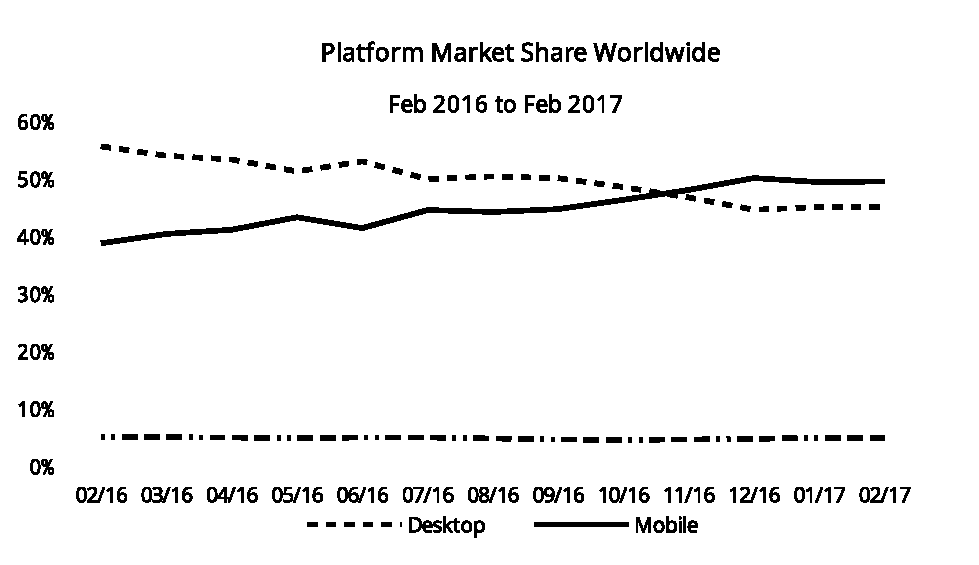
\includegraphics[width=1.00\textwidth]{platformMarketShare.eps}
  \caption{The distribution of platforms from around the world which browsed the
    internet from February, 2016 to February 2017. \fullcite{statCounter1}}
  \label{fig:StatCounter1}
\end{figure}
\begin{figure}
  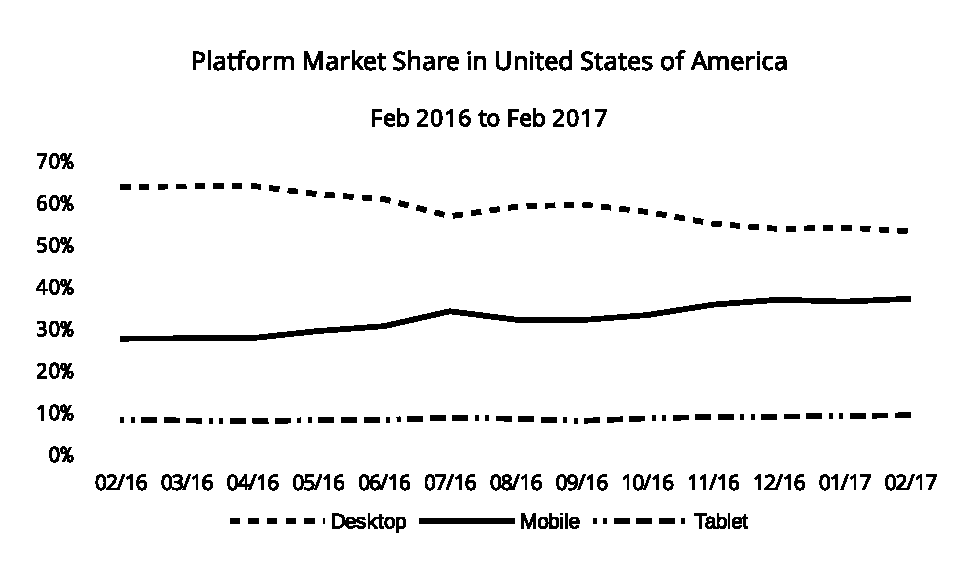
\includegraphics[width=1.00\textwidth]{platformMarketShareUS.eps}
  \caption{The distribution of platforms from the United States of America which browsed the
    internet from February, 2016 to February 2017. \fullcite{statCounter2}}
  \label{fig:StatCounter2}
\end{figure}
The result of not making one's web site friendly to mobile users is lessened when one examines the market share for only the United States of America, seen in Figure 2. Four web sites require Adobe Flash in order to experience content. These four web sites are leaving at least half of the users of the internet in the dark as Adobe has discontinued Flash development for mobile platforms.\autocite{adobeFlash} It is also quite surprising that only half of the artists have streaming audio on their web sites while every artist except six have streaming video. This may be an indication of the near-ubiquity of streaming video on the internet. It would have been interesting to see the shift from streaming audio to streaming video in the 2000s. \emph{Internet Archive}'s ``WaybackMachine'' may be a way in which to examine the developments of finger-style guitarists' web sites through the years.\autocite{internetArchive}
\begin{margintable}\centering
  \small
  \begin{tabular}{l l}\toprule
    \textsc{cms} & Number\\\midrule
    Bandzoogle & 4\\
    Hostbaby & 2\\
    Joomla & 1\\
    JuanPaSystems & 1\\
    ProdgWeb & 1\\
    Squarespace & 7\\
    Sumo & 1\\
    Truefire & 1\\
    WebsiteBuilder & 1\\
    Wix & 3\\
    Wordpress & 1\\\midrule
    Total & 23\\
    \bottomrule
  \end{tabular}
  \vspace{6pt}  
  \caption{Distribution of discernable Content Management Systems \textsc{cms} among the
    web sites of finger-style guitarists.} 
\end{margintable}
An area of particular interest to me was the manner in which these web sites managed their content. I was able to determine the Content Management Systems (\textsc{cms}) of 23 sites as seen in Table 3. The most represented \textsc{cms} is Squarespace with 7 artists followed by Bandzoogle at 4 and Wix at 3. I find this interesting because some of these \textsc{cms}'s integrate components into their systems which may assist an artist in the management of his or her web site. For instance, Bandzoogle assists in creating mobile-friendly web sites with a web store, newsletters, streaming services, blogs, and a gig calendar.\cite[12pt]{bandzoogle} The web sites which did not have any discernible manner in which to determine content creation may or may not have been created and managed with a \textsc{cms}.

One of the primary catalysts for this essay was to conduct a review of the distribution of sheet music within a digital finger-style domain. Almost every web site delivered their transcriptions in a different way. A few sites, such as Pierre Bensusans' had what appeared to be a custom built store. Others, such as Gareth Pearson, linked out to other venues such as CandyRat or Bandcamp. Many artists sold their products through PayPal in which the site redirected the customer to PayPal to make his or her purchase. Several sites, including Alex de Grassi's, delivered through a storefront created by their \textsc{cms}.

Each difference in the delivery of content can either enhance or detract from the user experience. This essay is only a survey, not a discussion, of expected graphical design components of a finger-style guitarist's web site.
\section{Transcription}
A distinguishing characteristic of the finger-style guitarist's website is a section of sheet music, scores, or transcriptions of the artist's works. This seems to be a unique component of the finger-style culture. Sadly, while the transcriptions are becoming marginally better than ascii-tab on the internet, the quality of the transcriptions produced by these musicians is generally not on par with the quality of playing or composition. This could be attributed to different factors, all of which are for another essay. Here I will discuss near-best practices for the production of finger-style transcriptions.
\subsection{Methods}
\label{sec:methods}
The primary method espoused by John Stropes of Stropes Editions, Ltd. is a double-impression method utilizing Finale and Adobe InDesign. The methods used in this document are as follows: XeLaTeX for the typesetting of this essay and the same double-impression method of Finale and Adobe InDesign used by Stropes Editions for the transcription. I also used FontForge to modify some of the fonts that I used in Finale.
\begin{figure*}\centering
        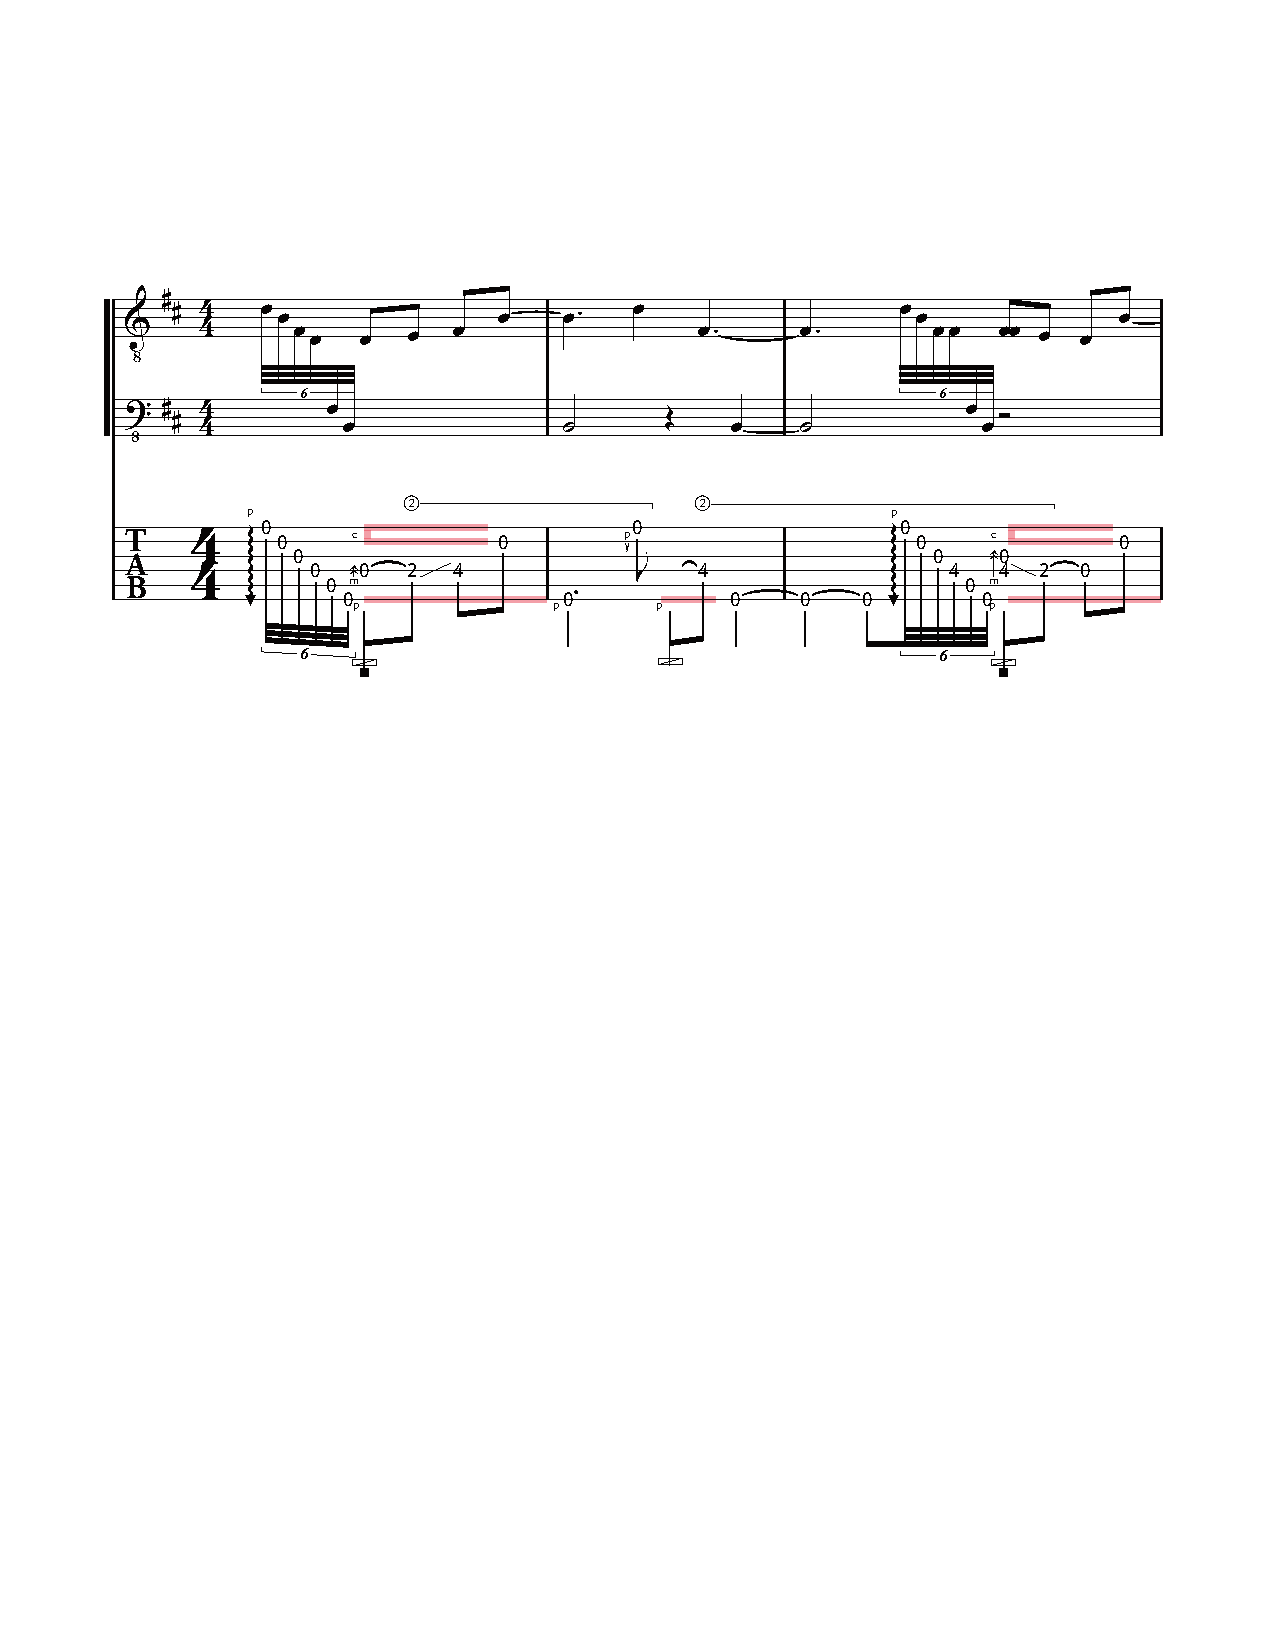
\includegraphics[width=1.00\textwidth]{watchTheTigerWalk20170326.pdf}
    \caption{``Watch the Tiger Walk'' by Rachael Carlson, mm. 1--2.}
    \label{fig:somthing}
  \end{figure*}
\subsection{Typography}
\label{sec:typography}

Stropes Editions, Ltd. has been at the forefront of the development of transcription and typesetting for finger-style guitar since the 1980s. These developments can be examined from a historical perspective starting with \emph{Twentieth Century Masters of Finger-Style Guitar}, \emph{Leo Kottke: Eight Songs}, and \emph{Michael Hedges: Rhythm, Sonority, Silence} to ``Ants'' and the unreleased grid notation for ``Madness.'' These examples represent pinnacles n the art of sheet music engraving for the guitar.  Due to these innovations, it can be difficult to reach beyond the conventions established. When the transcriptions from Stropes Editions are examined within a historical context one is able to tell that there is a sense that innovation is more important than tradition. This is an important distinction as it means that when confronted with the option to either adopt a new innovation or stay with a tradition, Stropes Editions seems to prefer to adopt that innovation. 

  While Stropes Editions prefers innovation, it can be difficult to produce a document which relies on the same innovations but uses a different visual aesthetic. I am reminded of a quote by the highly influential designer, Paul Rand, ``new becomes threatening, the old reassuring.'' While the design of Stropes Editions sheet music would not be considered bad, in fact they stand apart from all previous transcriptions in their beauty, they have established themselves as reassuring. The fonts used at Stropes Editions are Helvetica \textsc{lt} Std, \textsc{itc} Franklin Gothic and occasionally Times New Roman. It can be quite difficult to produce a score for finger-style guitar which does not either copy Stropes Editions or fall into the category of ugly music for the guitar. The difficulty of producing a unique voice within the field of music engraving is perhaps due to this feeling of reassurance. We are tasked with the necessity of simultaneously producing documents that are almost audible in their beauty while ensuring the maximum level of legibility. 
  
I have carefully chosen the typography of my transcriptions. It is designed for optimal legibility at small font sizes while ensuring the reader will not confuse one glyph for another.
  \begin{table}\centering
    \small
    \begin{tabular}{l l}\toprule
      Page Content  & Font \\\midrule
      Title & \emph{Garamond Premier Pro} Display Italic 28pt\\
      Tuning & \emph{EB Garamond} 12 Regular 10pt\\
      Octave Designation & \emph{EB Garamond} 12 Regular 10pt subscript\\
      Composer & \emph{EB Garamond} 12 Regular 10pt\\
      Clef & \emph{Adobe Garamond Pro} Bold 11pt\\
      Noteheads & \emph{Noto Sans} Regular 12pt\\
      Left-Hand Fingering & \emph{Noto Sans} Symbols 12pt\\
      Right-Hand Fingering & \emph{EB Garamond} 08 Regular 8pt\\
      Copyright and Page Numbers & \emph{EB Garamond} 08 Regular 8pt\\
      \bottomrule
  \end{tabular}
    \caption{Weights and sizes of fonts used in my transcriptions.}
\end{table}
Fonts that are designed based upon Claude Garamont (c. 1510 -- 1561) and Robert Granjon (1513 -- 1590) speak to me. Both Garamont and Granjon were French type designers and publishers in France. EB Garamond is an open source project directed by Georg Duffner based upon the ``\href{run:specimen.pdf}{Berner specimen},'' a document created by Frankfurt foundry Egelnolff-Berner in 1592 using type made by Garamont to sell their services.  The default numerical figures used in EB Garamond are old-style. This poses an issue when using this font with Finale as Finale is unable to interact with the OpenType features of a font, such as changing from old-style to lining figures. As such, I needed to modify a several of the font files of EB Garamond in FontForge in order to use lining numerals when appropriate. On the web site for EB Garamond, Duffner notes that he plans to design 18pt and 40pt varieties.\cite{duffner} Due to the current lack of a display version of EB Garamond I use Adobe's Garamond Premier Pro Display for the titles. This specimen does not contain bold examples. As such, neither does EB Garamond. For the \textsc{tab} clef I use Adobe Garamond Pro because it has a reasonable bold variation of the Garamond type. On the complete opposite end of the Garamond spectrum, for the noteheads and the left-hand fingering I use Google's Noto Sans. This font family was designed for the mobile market as a means to ensure that almost all of the more than 128,000 figures in \emph{The Unicode Standard} are present such that a user is able to see as many glyphs as possible with one font set. It is a humanist sans-serif based on Roboto, Droid Sans, and DIN.

There must to be a time when one makes a decision knowing all of the positives and negatives associated with that decision. It is at this point that it is more important that one makes \emph{a} decision than whether that decision is the best possible decision. I have vacillated between ten or so different fonts for my transcriptions. The decision of which font combination ensures readability while expressing an individual voice is an extremely difficult set of decisions. EB Garamond is a work in progress. It may be a better decision in the present to use Garamond Premier Pro due to its extent. However, I plan to contribute to the development of EB Garamond by developing the 10pt, 18pt, and 40pt optical sizes. I enjoy using Noto Sans because it contains circled numbers and letters --- {\symbolfont① ② ③ ④ Ⓣ}. The creation of these circled numbers and letters is possible within Finale; however, it takes a tremendous amount of time to ensure that the number or letter is displayed in the middle of the enclosure. A font which contains these circled glyphs solves this problem. It also introduces another problem as it does not contain negative numbers or letters which would be used for guide fingers. I believe that this is a small sacrifice.

\section{Web Site Development}
\label{sec:web-site-development}

The most visible component of this essay is the artist's web site. Based upon the information that I have gathered from this survey, I decided to move my web site to a \textsc{cms} called Squarespace. Among the pages with a discernible \textsc{cms}, seven artists used Squarespace. These were: Alex de Grassi, Graig D'Andrea, Jimmy Wahlsteen, Kaki King, Kevin Horrigan, Lucas Michailidis, and Peppino D'Agostino. The layout of these web sites were similar for some and quite dissimilar for others. D'Andrea and Horrigan seem to be using the same template. Wahlsteen's theme makes some of the text unreadable. King's web site has a major focus on a new album and the visual components of that album. D'Andrea and de Grassi each utilized Squarespace's commerce portal. This portal was a major component which affected my decision. Based upon personal interest, I purchased de Grassi's arrangement of ``St. James Infirmary'' through his web site. It was exceedingly easy to purchase this transcription.

The decision to move my web site operations over to Squarespace was not without careful discernment. I have had a bespoke web site for about five years. I know \textsc{html} and \textsc{css} enough to make me think that I should make and maintain my own web site. There are problems inherent to this which I will discuss later. There were two different \textsc{cms}'s that I was considering: the afore mentioned Squarespace and Bandzoogle. Bandzoogle is the only major contender with Squarespace in this field. It is tailored for especially to meet the demands of performing and recording musicians. There are others which compete with Squarespace; however, if the survey of finger-style guitarists can be used any sort of measure, HostBaby, Wix, and Wordpress are currently outliers. Squarespace integrates with Facebook in a manner which will help streamline my social media presence through directly posting to my Facebook page and by incorporating bandsintown.com as an events list. 

There were several necessary steps to take before the transition over to Squarespace could begin. I needed to ensure that the transition would be seamless. I contacted Squarespace inquiring about the process of transferring a domain from GoDaddy which was currently set to have email routed to Google. Squarespace responded that when the transfer of a domain is initiated only the necessary records are changed in order for the domain to have the correct server deliver the content to the user. All \textsc{mx} records stay the same. This would mean that the Google G Suite that I use for email would not receive any interruption in operation.

After I determined that it was going to be possible to switch to Squarespace with minimal interruption, I started a free 14-day trial in order to create and edit my theme. If I didn't create this free trial first, when I moved my domain over to Squarespace there would be a period of frantic content creation as the web site would be appearing to users as under construction. Several days into the trial, I felt that my web site was ready to transition. Within 24 hours the process was complete. Then I upgraded from the free trial to a paid membership. Finally, my Squarespace web site was live. To complete this process, I connected my PayPal and Stripe accounts to my Squarespace ecommerce page and uploaded a transcription of an arrangement that I made for Partita No. 3 in E Major: III. Gavotte en Rondeau by Johann Sebastian Bach. Within, six hours I had my first sale.

\section{``Watch the Tiger Walk''}
\label{sec:watch-tiger-walk}

It may not be necessary to mention the drastic changes that have affected the music industry in the last 20 years. I will, however, briefly discuss the factors which may have led to the rise of video as the primary means of the dissemination of music. The first steps of the change might be traced to the rise of the mp3 in the second half of the 1990s of which the small file size facilitated the distribution of music through the internet either through authorized sources such as mp3.com or unauthorized sources such as Napster. These first steps into the wide world cemented music's relationship to the internet. From my perspective, the next major change in the music industry was with YouTube, founded in 2005. We are still experiencing the repercussions of YouTube.

In order to partially keep up with the changes listed above, I have recorded the audio and video for ``Watch the Tiger Walk,'' an original composition. The video was recorded at 1920x1080 60p with a Panasonic ... and a matched pair of Beyerdynamic MC930 small diaphragm condenser microphones through the preamplifier on the camera. The audio was then processed in Logic Pro X. The video was rendered in Adobe Premiere Pro using the H. 264 codec.

\noindent \href{run:Road.mp3}{Audio}

\noindent\href{run:creativeCommons.mp4}{Video}

\section{Conclusions}
\label{sec:conclusions}

There can only be one conclusion to an essay such as this: there is no conclusion. The technologies involved in constructing both web sites and finger-style transcriptions is in a constant state of development. The prevalence of the mobile platform has become near-ubiquitous within the last five years. The manner in which finger-style guitar transcriptions are produced has changed drastically in the last thirty years. The software that is available to produce finger-style guitar transcriptions are at the users fingertips, a mere download away. While this software may not produce professional-grade transcriptions on the same level as an Stropes Editions transcription, they have helped begin the process of taking guitar tablature out of the dark ages of ascii-tab. It is not possible to conclude how the future of finger-style guitar is going pan out. What \emph{can} be concluded is that it is incredible to be a finger-style guitarist in an age in which finger-style guitar is experiencing a renaissance. There is a distinct possibility that someone I know may come across or benefit greatly from some new technology that cannot be imagined.

The work in the essay is truly a beginning. It was not possible at the outset to address each component of the digital life of a finger-style guitarist in the 21st century. Much still needs to be accomplished. Continued work needs to be done in these areas: a deep analysis of the typesetting of finger-style guitar tablature with the aim of establishing a reference work, 

\nocite{alexAnderson,alexDeGrassi,andrewWhite,andyMcKee,billyMcLaughlin,adamRafferty,calumGraham,cliveCarroll,craigDAndrea,evaAtmatzidou,ewanDobson,garethPearson,happyTraum,ianEthanCase,janetFeder,jimmyWahlsteen,jonGomm,kakiKing,kellyValleau,kevinHorrigan,leoKottke,lucaStricagnoli,lucasMich,masaakiKishibe,michaelChap,michaelGul,mikeDawes,murielAnders,peppino,peterCiluzzi,peterFinger,pierre,rayMontford,pino,spencerElliot,sunghaJung,thomasLeeb,timSparks,tommyEmmanuel,trevorGH,vickiGenfan}
% \bibliographystyle{chicagoa}
% \bibliography{bibliography}
\printbibliography
\clearpage

\section{Appendix 1}
\label{sec:appendix-1}


\begin{longtable}{p{0.2\textwidth} p{0.1\textwidth} p{0.2\textwidth} p{0.2\textwidth} p{0.2\textwidth} p{0.2\textwidth}}
  \caption[Web Site Data Set of Select Finger-Style Guitarists, pt. 1]{Web Site Data Set of Select Finger-Style Guitarists, pt. 1} \label{dataset1}\\

  \toprule
  \multicolumn{1}{p{0.1\textwidth}}{Artist} &
  \multicolumn{1}{p{0.2\textwidth}}{Status} &  
  \multicolumn{1}{p{0.2\textwidth}}{Claim to Legitimacy} &
  \multicolumn{1}{p{0.2\textwidth}}{Legitimacy Short-Form} &
  \multicolumn{1}{p{0.2\textwidth}}{Visual Display} &
  \multicolumn{1}{p{0.2\textwidth}}{Relation to Craft}\\ \midrule
  \endfirsthead

  \multicolumn{6}{c}
  {{\tablename\ \thetable{} -- continued from previous page}}\\
  \toprule
  \multicolumn{1}{p{0.1\textwidth}}{Artist} &
  \multicolumn{1}{p{0.2\textwidth}}{Status} &  
  \multicolumn{1}{p{0.2\textwidth}}{Claim to Legitimacy} &
  \multicolumn{1}{p{0.2\textwidth}}{Legitimacy Short-Form} &
  \multicolumn{1}{p{0.2\textwidth}}{Visual Display} &
  \multicolumn{1}{p{0.2\textwidth}}{Relation to Craft}\\ \midrule
  \endhead

  \midrule \multicolumn{6}{r}{{Continued on next page}}\\
  \endfoot

  \bottomrule
  \bottomrule
  \endlastfoot

  Adam Rafferty & Up-and-coming & auto playing video tries to establish his personal touch,  & Instructional & lesson-forward,  & open, he wants you to buy into his lessons\\
  Alex Anderson & Up-and-coming & seems to demonstrate this through having a harp guitar & Material & harp guitar forward & closed\\
  Alex de Grassi & Established & as a musician and a composer & Musical & picture of Alex front and center & open, workshops\\
  Andrew White & Up-and-coming & reviews of his music by important artists & Testimonial & picture-forward & closed\\
  Andy McKee & established & no overt claims to legitimacy & None & cute animated guitar player on homepage, mobile-friendly & closed\\
  Billy McLaughlin & established & focus on his recovery from focal dystonia & Inspirational & lots of pictures & open about focal dystonia, has videos of guitar instruction\\
Calum Graham & Up-and-coming & through YT views, through reviews by websites, luthiers, and artists & Testimonial & not very readable, Open Sans, page background is picture of Calum, mobile friendly & Open, there are links to set up Skype lessons with Calum, and videos of instruction on covers and originals\\
Clive Carroll & Established & tours & Musical & nice image of artist front and center & open, workshops\\
Craig D'Andrea & Up-and-coming & not demonstrating any sort of legitimacy & None & big fancy picture & closed\\
Eva Atmatzidou & Up-and-coming & a legitimate up and coming artist & Fresh & bad website, cheap, picture background & open\\
Ewan Dobson & Up-and-coming & video of “Time 2” seems to be his attempt to establish legitimacy & Musical & boring, with a great picture on the front page & open with Skype lessons\\
Gareth Pearson & Up-and-coming & Tommy Emmanuel quote & Testimonial & fancy, nice picture up front & closed\\
Happy Traum & established & as “Woodstock's own folk music legend” & Historical & nice picture of happy on front with good typography on page & open\\
Ian Ethan Case & Up-and-coming & a major focus on the double-neck guitar, lots of reviews, list of select previous performances & Testimonial, Musical & one picture which focuses on double-neck instrument,  & closed\\
Janet Feder & established & through a long career of composition & Musical & one page, nicely made, slick & closed\\
Jimmy Wahlsteen & Up-and-coming & no mention & None & illegible navbar,  & closed\\
Jon Gomm & established & reviews & Testimonial & cartoonish, reminds me of Heroes & open\\
Kaki King & established & new album & Musical & black with white and lots of color on her & master classes\\
Kelly Valleau & Up-and-coming & instructor first & Instructional & blog & open\\
Kevin Horrigan & Up-and-coming & review from Andy McKee & Testimonial & nice presentation website does not seem to be done & open\\
Leo Kottke & established & no mention & None & dark, grainy & closed\\
Luca Stricagnoli & Up-and-coming & through reviews & Testimonial & landing page is a big link to a video & closed\\
Lucas Michailidis & Up-and-coming & through reviews & Testimonial & legible,  & open\\
Masaaki Kishibe & established & lots of albums, its in Japanese mostly & Musical & a nice picture & closed\\
Michael Chapdelaine & established & “Professor of guitar” & Instructional & cheap, nice picture, bad colors, comic sans & open\\
Michael Gulezian & established & heavy on quotes from entities and individuals & Testimonial & heavy on images of Michael & closed\\
Mike Dawes & Up-and-coming & tours & Musical & lots of pictures of Mike & open\\
Muriel Anderson & established & legitimacy through connections & Testimonial & funny pictures of Muriel & open\\
Peppino D'Agostino & established & through a Leo Kkottke quote & Testimonial & picture heavy & open\\
Peter Ciluzzi & Up-and-coming & through tours and video performances & Musical & black text on white background & open\\
Peter Finger & established & reputation & Historical & emphasis on where he is playing next & closed\\
Pierre Bensusan & Established & through sponsorship, tour dates,  & ``Musical, 
Material'' & not mobile-friendly, desktop readable & Kinda closed, Offers residential seminars (in his home once a year)\\
Pino Forastiere & established & history and reviews & ``Historical, Musical'' & modern black on white & closed\\
Ray Montford & Up-and-coming & as a producer and engineer & Musical & looks like a blog template & closed\\
Spencer Elliott & Up-and-coming & as a candy rat artists & Associative & centers around pictures of artist and album artwork & closed\\
Sungha Jung & Up-and-coming & his youth & youthfulness & sort of looks like old apple website & closed\\
Thomas Leeb & Up-and-coming & studying west African traditional music.  & musical & hip, has his own logo,  & closed\\
Tim Sparks & established & awards, reviews & testimonial & ugly red & open wants you to buy into his shtick\\
Tommy Emmanuel & established & his imperfections are perfect & testimonial & slick, fonts are a little too small & closed\\
Trevor Gordon Hall & Up-and-coming & new album and video & musical & background from album artwork & open\\
Vicki Genfan & established & world music, claims she is a virtuoso & musical & small type good pictures & open\\
\end{longtable}
\clearpage
\section{Appendix 2}
\label{sec:appendix-2}


\begin{longtable}{l p{0.1\textwidth} l l l l l p{0.1\textwidth} l p{0.2\textwidth}}
  \caption[Web Site Data Set of Select Finger-Style Guitarists, pt. 2]{Web Site Data Set of Select Finger-Style Guitarists, pt. 2} \label{dataset1}\\

  \toprule
  \multicolumn{1}{l}{Artist} &
  \multicolumn{1}{p{0.1\textwidth}}{Mobile-Friendly?} &
  \multicolumn{1}{l}{Flash} &
  \multicolumn{1}{l}{https?} &
  \multicolumn{1}{l}{Audio} &
  \multicolumn{1}{l}{Video} &
  \multicolumn{1}{l}{Booking} &
  \multicolumn{1}{p{0.1\textwidth}}{Twitter Feed} &
  \multicolumn{1}{l}{Newsletter} &  
  \multicolumn{1}{p{0.1\textwidth}}{Newsletter How}\\ \midrule
  \endfirsthead

  \multicolumn{10}{c}
  {{\tablename\ \thetable{} -- continued from previous page}}\\
  \toprule
  \multicolumn{1}{l}{Artist} &
  \multicolumn{1}{p{0.1\textwidth}}{Mobile-Friendly?} &
  \multicolumn{1}{l}{Flash} &
  \multicolumn{1}{l}{https?} &
  \multicolumn{1}{l}{Audio} &
  \multicolumn{1}{l}{Video} &
  \multicolumn{1}{l}{Booking} &
  \multicolumn{1}{p{0.1\textwidth}}{Twitter Feed} &
  \multicolumn{1}{l}{Newsletter} &  
  \multicolumn{1}{p{0.1\textwidth}}{Newsletter How}\\ \midrule  
  \endhead

  \midrule \multicolumn{10}{r}{{Continued on next page}}\\
  \endfoot

  \bottomrule
  \bottomrule
  \endlastfoot

  Adam Rafferty & no & no & yes & no & no & yes & no & yes & with a disruptive popup\\
  Alex Anderson & yes & no & no & no & no & no & no & yes & bandzoogle.com\\
  Alex de Grassi & yes & no & yes & yes & yes & no & no & no & \\
  Andrew White & no & no & no & yes & no & yes & no & no & \\
  Andy McKee & yes & no & no & no & yes & yes & no & yes & TBD\\
  Billy McLaughlin & yes & no & yes & no & yes & yes & yes & yes & constant contact\\
  Calum Graham & yes & no & no & yes & yes & yes & yes & yes & bandzoogle.com\\
  Clive Carroll & yes & no & yes & no & yes & yes & no & yes & mailchimp\\
  Craig D'Andrea & yes & no & yes & no & yes & yes & no & yes & squarespace\\
  Eva Atmatzidou & no & no & yes & no & yes & yes & no & no & \\
  Ewan Dobson & yes & no & yes & no & yes & no & no & no & \\
  Gareth Pearson & no & no & yes & no & yes & yes & no & yes & WIX\\
  Happy Traum & no & no & no & no & yes & no & no & no & \\
  Ian Ethan Case & no & no & yes & yes & yes & yes & no & yes & MailChimp\\
  Janet Feder & yes & no & yes & yes & no & yes & yes & no & \\
  Jimmy Wahlsteen & yes & no & yes & no & no & yes & no & no & \\
  Jon Gomm & no & no & yes & yes & yes & yes & no & yes & bandzoogle.com\\
  Kaki King & yes & no & yes & yes & yes & yes & no & yes & \\
  Kelly Valleau & no & no & yes & no & yes & no & no & no & \\
  Kevin Horrigan & yes & no & yes & no & yes & yes & no & no & \\
  Leo Kottke & no & no & yes & no & no & yes & no & no & \\
  Luca Stricagnoli & yes & no & yes & yes & yes & yes & no & no & \\
  Lucas Michailidis & yes & no & yes & yes & yes & no & no & yes & MailChimp \\
  Masaaki Kishibe & no & yes & yes & yes & yes & no & no & no & \\
  Michael Chapdelaine & no & no & yes & yes & yes & yes & no & no & \\
  Michael Gulezian & no & yes & no & yes & yes & yes & no & yes & manual from Michael\\
  Mike Dawes & no & no & yes & yes & yes & yes & no & yes & \\
  Muriel Anderson & yes & no & yes & yes & yes & yes & no & yes & \\
  Peppino D’Agostino & yes & no & yes & yes & yes & yes & no & yes & mailchimp\\
  Peter Ciluzzi & no & no & yes & yes & yes & yes & no & no & \\
  Peter Finger & no & no & yes & no & yes & yes & no & no & \\
  Pierre Bensusan & no & no & no & yes & yes & yes & no & no & \\
  Pino Forastiere & yes & no & yes & no & yes & yes & no & no & \\
  Ray Montford & no & no & yes & no & yes & yes & yes & yes & MailChimp\\
  Spencer Elliott & yes & no & yes & no & yes & no & no & no & \\
  Sungha Jung & no & no & yes & no & yes & no & no & no & \\
  Thomas Leeb & yes & no & yes & yes & yes & yes & no & no & \\
  Tim Sparks & no & yes & yes & yes & yes & yes & no & no & \\
  Tommy Emmanuel & yes & no & yes & no & yes & no & no & yes & a fan club\\
  Trevor Gordon Hall & yes & yes & yes & no & yes & yes & no & no & \\
  Vicki Genfan & no & no & yes & yes & yes & yes & no & yes & mail-dog.com\\

\end{longtable}
\clearpage
\section{Appendix 3}
\label{sec:appendix-3}


\begin{longtable}{p{0.2\textwidth} p{0.3\textwidth} p{0.1\textwidth} p{0.2\textwidth} p{0.2\textwidth} p{0.3\textwidth}}
  \caption[Web Site Data Set of Select Finger-Style Guitarists, pt. 3]{Web Site Data Set of Select Finger-Style Guitarists, pt. 3} \label{dataset3}\\

  \toprule
  \multicolumn{1}{p{0.1\textwidth}}{Artist} &
  \multicolumn{1}{p{0.3\textwidth}}{Contact} &  
  \multicolumn{1}{p{0.1\textwidth}}{Social Media} &
  \multicolumn{1}{p{0.2\textwidth}}{Tour Dates} &
  \multicolumn{1}{p{0.2\textwidth}}{News} &
  \multicolumn{1}{p{0.3\textwidth}}{Transcription}\\ \midrule
  \endfirsthead

  \multicolumn{6}{c}
  {{\tablename\ \thetable{} -- continued from previous page}}\\
  \toprule
  \multicolumn{1}{p{0.1\textwidth}}{Artist} &
  \multicolumn{1}{p{0.3\textwidth}}{Contact} &  
  \multicolumn{1}{p{0.1\textwidth}}{Social Media} &
  \multicolumn{1}{p{0.2\textwidth}}{Tour Dates} &
  \multicolumn{1}{p{0.2\textwidth}}{News} &
  \multicolumn{1}{p{0.3\textwidth}}{Transcription}\\ \midrule
  \endhead

  \midrule \multicolumn{6}{r}{{Continued on next page}}\\
  \endfoot

  \bottomrule
  \bottomrule
  \endlastfoot
  
  Adam Rafferty & manual it appears & FB, G+, Pinterest, tumblr, TW, YT & bandsintown.com & blog style with comments & pushing for his new website StudyWithAdam.com;   he doesn’t “distribute unlicensed sheet music, tabs or PDFS - PERIOD.”\\
  Alex Anderson & messaging through website & FB, TW, SC, YT, IG & none in the future & on main page only, blog style with comments & none\\
  Alex de Grassi &  & FB, TW, SC,  & seem to be manually entered &  & \$6.50 / transcription, through square space pdf delivered instantly\\
  Andrew White & most likely a friend or colleague not a company & FB, YT, TW, IG & bandsintown.com & Blog style posts with comments section & cartscheckout.com and PayPal\\
  Andy McKee & northstar artists & FB, TW, IG, YT & bandsintown.com  & short captions for pictures & \$2.50/transcription, links out to missinglinkshop.com\\
  Billy McLaughlin & north star artists Kevin & fb, tw, g+, pinterest, linkedIn,  & appears to be custom made & blog style without comments & link to stropes.com\\
  Calum Graham & Feldman Agency out of Canada & FB, IG, YT, TW, SC & bandsintown.com & Blog style posts with comments section & \$5C/“guitar tab” delivered through pdf, links out to PayPal\\
  Clive Carroll & CPR Entertainment & tiny FB, TW & seem to be manually entered & none & not much, through paypal, \$3.50 euros\\
  Craig D'Andrea & Cadet Music Presents & FB, TW, IG, YT & yes, none currently,  & none & sold through squarespace\\
  Eva Atmatzidou & contact her directly & FB &  & non & sold through candyrat\\
  Ewan Dobson &  & TW, FB, YT & none currently, manual & non & sold through fastspring.com\\
  Gareth Pearson & pavel lychagin, his manager & IG, FB, YT, VK (?) & auto through something I can’t see & none & sold through candyrat\\
  Happy Traum &  &  & appear to be manually entered by someone & blog style & sold through homespun \\
  Ian Ethan Case & through booking@ianethan.com & FB, TW, YT & yes, appears to be manually entered & on home page, pithy including pictures and videos & none\\
  Janet Feder & rjpr music & FB, TW, BC &  & blog style & non, store is on Bandcamp\\
  Jimmy Wahlsteen & booking in germany and scandanavia & TW, FB, IG,  & none currently, manual & blog style & through candy rat\\
  Jon Gomm & manager & FB, TW, YT, MySpace & zoogle & blog style with comments & through paypal\\
  Kaki King & Cadenza Plus & TW, IG, SC, YT, FB & bandsintown.com & old news, appears manual & through backstreetmerch.com\\
  Kelly Valleau &  &  &  & its a blog & through musicnotes.com which seems to allow for proper licensing as well\\
  Kevin Horrigan & through form on site & FB, IG, SC, YT, TW &  &  & \\
  Leo Kottke & Fred Bohlender Paradigm &  & manually entered &  & \\
  Luca Stricagnoli & through form on site & FB, YT, & none currently, &  & none\\
  Lucas Michailidis & contact through form on site & FB &  &  & available through stropes and candy rat\\
  Masaaki Kishibe & its in japanese &  &  &  & \\
  Michael Chapdelaine & through form on site & TW, IG & manually entered &  & through paypal, each transcription has a video\\
  Michael Gulezian & through Michael & I know that he has FB and YT but it is not easily found on website & appear to be hand entered & old news appears to be manually entered & Links out to Stropes editions\\
  Mike Dawes & through form on site & TW, FB, YT & bandsintown.com & Blog style posts with comments section & through candy rat and through PayPal\\
  Muriel Anderson & through related person &  &  & blog style without comments & music will be emailed within 24 hours\\
  Peppino D’Agostino & no booking in the states &  & bandsintown.com &  & individual transcriptions sold through e-junkie.com, books sold through alfred.com and amazon.com\\
  Peter Ciluzzi & booking@ & FB, TW, G+, PNT, LINK, YT & bandsintown &  & link to candy rat\\
  Peter Finger & Acoustic Music GmbH \& Co & FC, MySpace, last.fm, YT & manually entered & & \\
  Pierre Bensusan & Lewis Media Relations \& Live Entertainment Planning, contact through website & links to FB, TW, YT in two different locations & bandsintown.com & blog-style posts with comments section & through custom built site, pdf 20 euros for 12 tunes\\
  Pino Forastiere & through stefania & FB YT  & out of date in concerts section, up to date in news section & Blog style posts with comments section & sold through PayPal\\
  Ray Montford & contact ray &  & manually entered &  & none\\
  Spencer Elliott & through form on site & FB, TW, G+, Pnt & manually entered &  & tabs’ through candy rat\\
  Sungha Jung &  &  & old manual &  & \\
  Thomas Leeb & through form on site &  & probably through bandzoogle & blog style without comments & through bandcamp, transcriptions will be sent within 48 hours, they are watermarked and password protected\\
  Tim Sparks & through him @aol.com & FB, TW, YT & some stupid thing through reverbnation that doesn’t work (it requires flash) &  & through paypal\\
  Tommy Emmanuel &  & FB, TW, IG &  & blog style without post & shopify.com\\
  Trevor Gordon Hall & Cadet Music Presents & FB, IG, TW, YT & through some service &  & broken\\
  Vicki Genfan & contact a private person & FB, TW, MS, YT & google calendar & blogstyle without comments & nothing\\
  
\end{longtable}
FB: Facebook; TW: Twitter; SC: SoundCloud; YT: YouTube; IG: Intagram; G+: Google+; BC: Bandcamp; PNT: Pinterest; LINK: LinkedIn; MS: MySpace.\\

\clearpage
\section{Appendix 4}
\label{sec:appendix-4}


\begin{longtable}{p{0.25\textwidth} p{0.25\textwidth} p{0.3\textwidth} p{0.2\textwidth} p{0.4\textwidth}}
  \caption[Web Site Data Set of Select Finger-Style Guitarists, pt. 4]{Web Site Data Set of Select Finger-Style Guitarists, pt. 4} \label{dataset4}\\

  \toprule
  \multicolumn{1}{p{0.25\textwidth}}{Artist} &
  \multicolumn{1}{p{0.25\textwidth}}{Record Label} &  
  \multicolumn{1}{p{0.3\textwidth}}{Nameserver} &
  \multicolumn{1}{p{0.2\textwidth}}{Probable Host or \textsc{cms}} &
  \multicolumn{1}{p{0.4\textwidth}}{Notes} \\ \midrule
  \endfirsthead

  \multicolumn{5}{c}
  {{\tablename\ \thetable{} -- continued from previous page}}\\
  \toprule
  \multicolumn{1}{p{0.25\textwidth}}{Artist} &
  \multicolumn{1}{p{0.25\textwidth}}{Record Label} &  
  \multicolumn{1}{p{0.3\textwidth}}{Nameserver} &
  \multicolumn{1}{p{0.2\textwidth}}{Probable Host or \textsc{cms}} &
  \multicolumn{1}{p{0.4\textwidth}}{Notes} \\ \midrule
  \endhead

  \midrule \multicolumn{5}{r}{{Continued on next page}}\\
  \endfoot

  \bottomrule
  \bottomrule
  \endlastfoot
  Adam Rafferty &  & domaincontrol.com & sumo & starts with a popup for a mailing list\\
  Alex Anderson & candyrat & sitezoogle.com & bandzoogle & crowd=funded his latest album\\
  Alex de Grassi & indie & squarespace worldnic.com & squarespace & \\
  Andrew White & candyrat & Rook Media rookdns.com & wix & \\
  Andy McKee & CGP sounds & wix.com & wix & signed to CGP records (tommy emmanuel)\\
  Billy McLaughlin &  & go daddy worldnic.com &  & \\
  Calum Graham & CandyRat & sitezoogle.com & bandzoogle & An EPK which highlights his YouTube celebrity\\
  Clive Carroll &  & iPage fatcow.com &  & \\
  Craig D'Andrea &  & Squarespace ipower.com & squarespace & It looks like Craig D’Andrea is taking a break or something, this would be a good time to have a blog or news section.\\
  Eva Atmatzidou & candyrat & Google googleusercontent.com &  & \\
  Ewan Dobson & candy rat and indie & go daddy domaincontrol.com & juanpasystems & \\
  Gareth Pearson & candyrat & wixdns.net & wix & \\
  Happy Traum &  & Amazon designinterventionsites.com &  & \\
  Ian Ethan Case & CandyRat & hostbaby.com & hostbaby & stage plot, publicity photos, press kit includes bio, endorsements, and reviews; CDs sold through bandcamp and candyrat\\
  Janet Feder & indi? & latisys-denver electricstores.com &  & \\
  Jimmy Wahlsteen & candyrat & Squarespace loopia.se & squarespace & \\
  Jon Gomm & performing chimp records & RackSpace sitezoogle.com & bandzoogle & \\
  Kaki King &  & Squarespace register.com & squarespace & \\
  Kelly Valleau & candyrat & Weebly domaincontrol.com &  & really just seams to be a blog by the artist\\
  Kevin Horrigan &  & squarespace domaincontrol.com & squarespace & seems to be not done yet\\
  Leo Kottke &  & godaddy colorave.com &  & \\
  Luca Stricagnoli & candyrat & KPNQWest Italia netsons.com &  & \\
  Lucas Michailidis & candyrat & Squarespace jumbo.net.au & squarespace & \\
  Masaaki Kishibe &  & Sakura Internet dns.ne.jp &  & \\
  Michael Chapdelaine & they all look to be self-released & Cedant Web Hosting earthlink.net &  & would have been a professional website in the 2000s\\
  Michael Gulezian & timbrelinemusic.com many different companies called timbreline & ebusiness32.com &  & video streaming is really old and out-dated\\
  Mike Dawes & candy rat records & 1\&1 1and1-dns.com & word press & \\
  Muriel Anderson &  & worldnic.com &  & \\
  Peppino D’Agostino &  & squarespace domaincontrol.com & squarespace & \\
  Peter Ciluzzi & candyrat & webhostingpad.com &  & \\
  Peter Finger &  & Neue Medien Muennich kasserver.com &  & \\
  Pierre Bensusan & DADGAD Music & cyber host pro hostingsystems.co.uk &  & An EPK which tries to sell his latests CD\\
  Pino Forastiere & candy rat and indie & Aruba S.p.A. - Shared Hosting and Mail services technorail.com & prodgweb & \\
  Ray Montford & CandyRat & dreamhost.com & joomla & \\
  Spencer Elliott & CandyRat & go daddy domaincontrol.com & WebsiteBuilder & \\
  Sungha Jung &  & Lg Dacom Kidc nsgodo.com &  & he has a forum on his site which is populated by bots\\
  Thomas Leeb & indie & RackSpace domaincontrol.com & bandzoogle & \\
  Tim Sparks & CandyRat and Tzadik & dreamhost.com &  & annoying autoplaying video\\
  Tommy Emmanuel & CGP sounds & defense.net worldnic.com &  & \\
  Trevor Gordon Hall & through CDBaby & Integra Telecom hostbaby.com & hostbaby & \\
  Vicki Genfan &  & WideOpenWest domaincontrol.com & truefire.com & \\
  

  \end{longtable}
\end{document}
%%% Local Variables:
%%% mode: latex
%%% TeX-master: t
%%% End:
